
Como ya adelantamos brevemente en el apartado anterior, para la generacion de oraciones para la sintesis utilizamos Festvox y Festival. Al igual que con las trancripciones foneticas, estas herramientas nos permitirán traducir oraciones grafemicas (texto) a una lista de fonemas y metadata utilizados por HTK para sintetizar audio.

El primer desafío que se presenta es que estos repertorios fonéticos no tienen un mapeo directo entre el inglés y el castellano: por ejemplo con el repertorio fonético de festvox en castellano, existen tres fonos distintos para la /i/, decisión que proviene de la necesidad de poder diferenciar la /i/ acentuada de la no acentuada  y de aquella presente en los diptongos: /ia/, /ie/, /io/, /iu/.

\begin{table}
\centering
%\setlength{\tabcolsep}{6pt} % default value is 6pt
\caption{Repertorios Foneticos utilizados por Festvox para Inglés y Castellano}
\begin{minipage}[t]{0.3\textwidth}
\begin{tabular}[t]{cc}
\toprule
Castellano \\
\midrule
a & ll \\
a1&  m  \\
b & n  \\
ch&  ny \\
d & o  \\
e & o1 \\
e1&  p  \\
f & r  \\
g & rr \\
i & s  \\
i0&  t  \\
i1&  u  \\
k & u0 \\
l & u1 \\
\bottomrule
\end{tabular}
\end{minipage}
\begin{minipage}[t]{0.3\textwidth}
\begin{tabular}[t]{cc}
\toprule
Inglés \\ 
\midrule
 aa & jh\\
 ae & k \\
 ah & l \\
 ao & m \\
 aw & n \\
 ax & ng\\
 ay & ow\\
 b  &oy\\
 ch & p \\
 d  &r \\
 s  &sh\\
 dh & t\\
 eh & th \\
 er & uh \\
 ey & uw \\
 f  &v\\
 g  &w\\
 hh & y\\
 ih & z\\
 iy & zh \\
\bottomrule
\end{tabular}
\end{minipage}
\end{table}

De aquí surgen varios problemas. El primero es que festival utiliza el mismo simbolo para dos fonos distintos. De esta manera, la /g/ en castellano es suena mucho mas disminuida que la /g/ del repertorio inglés, aunque ambas sean descritas como un fono oclusivo velar sonoro. Acá la cagué esto no era así =(.

\verEnElCorpus

De esto, surge el siguente problema: cómo sintetizar oraciones en castellano utilizando un repertorio fonético en inglés, donde incluso la cantidad de fonos es diferente. La manera que encontramos de abordar esto fue confeccionando de manera perceptual una tabla donde cada fonema del castellano estuviera mapeado a uno del inglés. En otras palabras, antes del entrenamiento del modelo, tomamos los fonos generados por festival para el corpus en inglés y los reemplazamos con fonos del castellano de la manera ilustrada en la tabla 2.
\begin{table}
\centering
%\setlength{\tabcolsep}{6pt} % default value is 6pt
\caption{Mapeo Fonético}
\begin{minipage}[t]{0.3\textwidth}
\begin{tabular}[t]{c|c}
\toprule
Inglés & Castellano \\
\midrule
ae & a\\  
aa & a1\\  
b & b\\  
ch & ch\\  
d & d\\  
dh & d\\  
eh & e\\  
el & e1\\  
f & f\\  
hh & g\\  
iy & i\\  
%FALTA i0
ih & i1\\  
k & k\\  
l & l\\  
jh & ll\\  
m & m\\  
n & n\\  
nx & n\\  
ao & o\\  
ou & o1\\  
p & p\\  
r & r/rr\\  
\bottomrule
\end{tabular}
\end{minipage}
\begin{minipage}[t]{0.3\textwidth}
\begin{tabular}[t]{c|c}
\toprule
Inglés & Castellano \\ 
\midrule
s & s\\  
t & t\\  
uw & u\\  
w & u0\\  
uh & u1\\  
dx & -\\  
em & -\\  
en & -\\  
er & -\\  
ei & -\\  
g & -\\  
hv & -\\  
ng & -\\  
th & -\\  
v & -\\  
y & -\\  
sh & -\\  
zh & -\\  
z  & -\\  
\bottomrule
\end{tabular}
\end{minipage}
\end{table}

Por otro lado para varios fonos tuvimos que hacer reglas especiales ya que no contábamos con ningun fono del inglés lo suficientemente similar. Así,  para el fono ny (ñ o \textltailn, en ipa) colapsamos las apariciones del fono /n/ seguido de /j/. Si bien esta solución puede parecer algo forzada, ya que estamos generando de manera casera fonos a partir de otros, consideramos que esto se aproxima en cierta medida a la manera real en la que un hablante no nativo aprende un idioma con una carga fonética diferente al suyo. Citando un extracto del trabajo \textit{Transcription of Spanish and Spanish-Influenced English, Brian Goldstein, Temple University}\cite{spanishInfluencedEnglish}:

\begin{center}
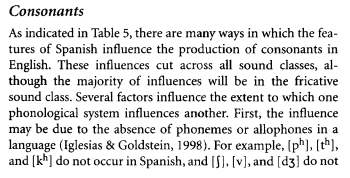
\includegraphics[scale=0.6]{imagenes_investigacion/consonantes1.png}
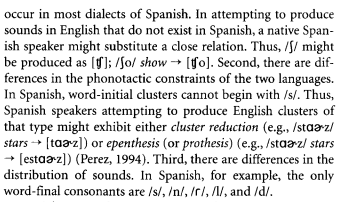
\includegraphics[scale=0.6]{imagenes_investigacion/consonantes2.png}
\end{center}

Visto desde nuestra perspectiva, una persona que aprende una nueva lengua, realiza una aproximación entre los fonos conocidos y los fonos `objetivo' de la nueva lengua.

De manera similar el inglés carece del fono vibrante múltiple alveolar sordo /\textipa{r}/ (\textit{perro}) y dado que el fono /\textipa{R}/(\textit{pero})  ya estaba siendo utilizado, no podíamos realizar un mapeo tan directo. Como sulución tomamos la mitad de los fonos /\textipa{R}/ y los reemplazamos con /\textipa{r}/. Un problema similar surge del fono /g/, que si bien existe en inglés, al utilizarlo para sintetizar oraciones sonaba antinatural para un hablante anglosajón. Con el objetivo de suavizar el sonido tomamos el fono de la /g/ y lo mapeamos a un fono que no fuera utilizado y tomamos los fonos etiquetados con /hh/ del inglés y los remplazamos con el /g/ del castellano.

Aquellos fonos que consideramos suficientemente disímiles del castellano, como es el caso de la /sh/, /z/, etc los mapeamos a caracteres que no interfirieran para el entrenamiento ya que no los utilizaremos para la síntesis de oraciones en castellano.

Con este mapeo podemos utilizar el corpus en ingles para sintetizar oraciones en castellano, aunque como es de esperar, dado que el corpus de entrenamiento es tan distinto de las oraciones que queremos sintetizar (Cuestiones como que las combinaciones de fonemas del ingles y el castellano son diferentes, las reglas prosodicas y las acentuaciónes vocalicas difieren entre los idiomas) los audios sitetizados resultan incomprensibles.

% mapeo utilizado mostrar.
% el etiquetado de cmu\_arctic es en inglés y mapeando al castellano.